%%%%%%%%%%%%%%%%%%%%%%%%%%%%%%%%%%%%%%%%%
% Short Sectioned Assignment
% LaTeX Template
% Version 1.0 (5/5/12)
%
% This template has been downloaded from:
% http://www.LaTeXTemplates.com
%
% Original author:
% Frits Wenneker (http://www.howtotex.com)
%
% License:
% CC BY-NC-SA 3.0 (http://creativecommons.org/licenses/by-nc-sa/3.0/)
%
%%%%%%%%%%%%%%%%%%%%%%%%%%%%%%%%%%%%%%%%%

%----------------------------------------------------------------------------------------
%	PACKAGES AND OTHER DOCUMENT CONFIGURATIONS
%----------------------------------------------------------------------------------------

\documentclass[paper=letter, fontsize=11pt]{scrartcl} % A4 paper and 11pt font size

\usepackage[T1]{fontenc} % Use 8-bit encoding that has 256 glyphs
% \usepackage{fourier} % Use the Adobe Utopia font for the document - comment this line to return to the LaTeX default
\usepackage[english]{babel} % English language/hyphenations
\usepackage{amsmath,amsfonts,amsthm} % Math packages

\usepackage{graphicx}
\usepackage{caption}
\usepackage{subcaption}

\usepackage{sectsty} % Allows customizing section commands
\allsectionsfont{\centering \normalfont\scshape} % Make all sections centered, the default font and small caps

\usepackage{fancyhdr} % Custom headers and footers
\pagestyle{fancyplain} % Makes all pages in the document conform to the custom headers and footers
\fancyhead{} % No page header - if you want one, create it in the same way as the footers below
\fancyfoot[L]{} % Empty left footer
\fancyfoot[C]{} % Empty center footer
\fancyfoot[R]{\thepage} % Page numbering for right footer
\renewcommand{\headrulewidth}{0pt} % Remove header underlines
\renewcommand{\footrulewidth}{0pt} % Remove footer underlines
\setlength{\headheight}{13.6pt} % Customize the height of the header

\numberwithin{equation}{section} % Number equations within sections (i.e. 1.1, 1.2, 2.1, 2.2 instead of 1, 2, 3, 4)
\numberwithin{figure}{section} % Number figures within sections (i.e. 1.1, 1.2, 2.1, 2.2 instead of 1, 2, 3, 4)
\numberwithin{table}{section} % Number tables within sections (i.e. 1.1, 1.2, 2.1, 2.2 instead of 1, 2, 3, 4)

\setlength\parindent{0pt} % Removes all indentation from paragraphs - comment this line for an assignment with lots of text

%----------------------------------------------------------------------------------------
%	TITLE SECTION
%----------------------------------------------------------------------------------------

\newcommand{\horrule}[1]{\rule{\linewidth}{#1}} % Create horizontal rule command with 1 argument of height

\title{	
\normalfont \normalsize 
\textsc{Missouri University of Science and Technology \\ Department of Mechanical and Aerospace Engineering} \\ [25pt] % Your university, school and/or department name(s)
\horrule{0.5pt} \\[0.4cm] % Thin top horizontal rule
\huge Structures II: Final Project \\ % The assignment title
\horrule{2pt} \\[0.5cm] % Thick bottom horizontal rule
}

\author{Mitchell Wainwright \\ Ryan Krattiger} % Your name

\date{\normalsize\today} % Today's date or a custom date

\begin{document}

\maketitle % Print the title

%----------------------------------------------------------------------------------------
%	PROBLEM 1
%----------------------------------------------------------------------------------------

\section{Editing Solver Code}

The edited code is available in the github repository found at: \\\\
\textit{https://github.com/rjk9w5/FEM\_project} 


\begin{figure}[h]
\centering
	\begin{subfigure}[b]{0.45\textwidth}
		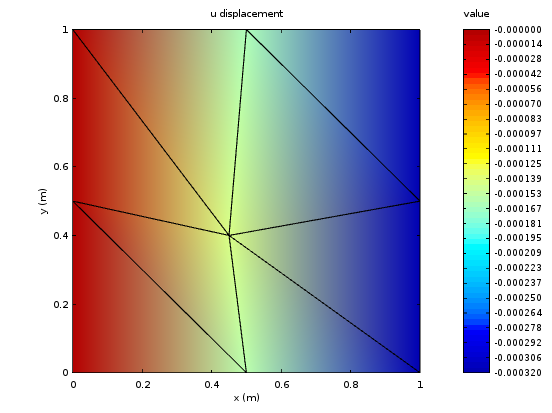
\includegraphics[width=\textwidth]{patchu.png}
		\caption{v displacement distribution}
		\label{fig:patchu}
	\end{subfigure}
	\hfill
	\begin{subfigure}[b]{0.45\textwidth}
		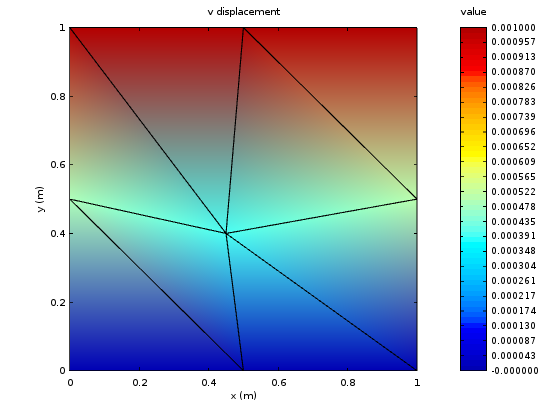
\includegraphics[width=\textwidth]{patchv.png}
		\caption{v displacement distribution}
		\label{fig:patchv}
	\end{subfigure}
	\caption{PatchTest.m output figures}
\end{figure}

\paragraph{Predicted Results from Patch Test}
The results expected from running the patch test come from the definitions of strain (eq. \ref{eq:axstraindef}) and Poisson's ratio (eq.\ref{eq:poissonrat}). Because the element is not being subjected to any shear forces there should be no $\epsilon_{xy}$ term. The consequent preditions are tabulated in table \ref{tab:patchtab}. It can be seen here that the results match exactly for both the $\epsilon_{xx}$ and $\epsilon_{yy}$ and are very nearly zero for $\epsilon_{xy}$. The output figures for u and v displacements can be seen in fig. \ref{fig:patchu} and fig. \ref{fig:patchv} respectively.

\begin{equation} \label{eq:axstraindef}
\epsilon_{yy} = \frac{v}{L}
\end{equation}
where v = 0.001 and L = 1. 

\begin{equation} \label{eq:poissonrat}
\nu = - \frac{\epsilon_{xx}}{\epsilon_{yy}}
\end{equation}
where $\nu = 0.32$.

\begin{table}[h]
\centering
	\begin{tabular}{c c c}
		& Predicted & Actual \\
		\hline
		$\epsilon_{xx}$ & -0.00032 & -0.00032 \\
		$\epsilon_{yy}$ & 0.001 & 0.001 \\
		$\epsilon_{xy}$ & 0 & $\approx 10^{-20}$ \\
		\hline
	\end{tabular}
\caption{Predicted and Actual results from running PatchTest.m}
\label{tab:patchtab}
\end{table}
	

%----------------------------------------------------------------------------------------
%	PROBLEM 2
%----------------------------------------------------------------------------------------
\pagebreak
\section{Dog-Bone in Uniaxial Tension}

%------------------------------------------------
The Young modulus (E) was calculated for various lengths of L where $L = \beta A$. 'A' is a constant, and $\beta$ was varied as 0.2, 0.5, 1, 2, and 5. The actual Young modulus was 70 GPa. The results are tabulated in table \ref{tab:q2table1} and shown graphically in fig. \ref{fig:q2fig1} and \ref{fig:q2fig2}. \\
\\
It can be seen that the Young modulus is within the desired tolerance of 10\% when the length is 10x the cross-sectional area. \\
\\

\begin{table}[!ht]
\centering
	\begin{tabular}{c c c}
		 $\beta$ & E [GPa] & \% error \\
		 \hline
		 0.2 & 14.48 & 79.31 \\
		 0.5 & 27.67 & 60.48\\
		 1 & 39.23 & 43.95\\
		 2 & 50.64 & 27.65\\
		 5 & 60.71 & 13.28\\
		 10 & 65.02 & 7.119\\
		\hline
	\end{tabular}
\caption{Tabulated Results for Calculated Young modulus}
\label{tab:q2table1}
\end{table}

\begin{figure}[h]
\centering
	\begin{subfigure}[b]{0.45\textwidth}
		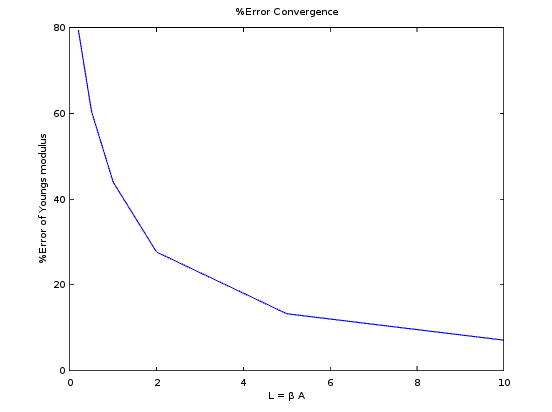
\includegraphics[width=\textwidth]{q2_error.png}
		\caption{Plot of \%error of calculated Young modulus}
		\label{fig:q2fig1}
	\end{subfigure}
	\hfill
	\begin{subfigure}[b]{0.45\textwidth}
		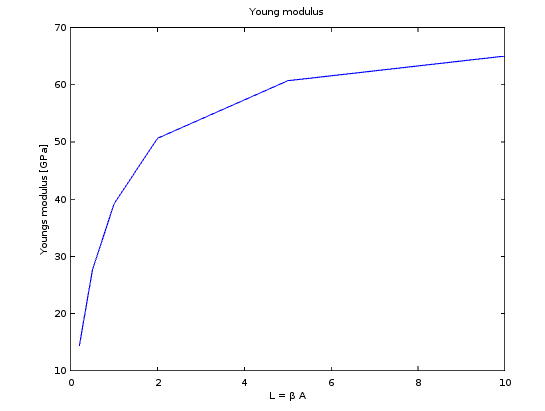
\includegraphics[width=\textwidth]{q2_youngmod.png}
		\caption{Plot of calculated Young modulus}
		\label{fig:q2fig2}
	\end{subfigure}
	\caption{\%Error and value of apparent Young modulus versus gage length}
\end{figure}

The reason an error occurs in the calculation of the Young modulus is a result of the numerical errors from running the simulation. The longer the dog-bone specimen becomes the closer it matches the actual value. This can be attested to the observations made in St. Venant's principle.
\\\\
\textit{"... the difference between the effects of two different but statically equivalent loads becomes very small at sufficiently large distances from load."}
\\\\
As the length of the rod increases, the distance from the load increases, and the difference between the results obtained in each iteration becomes smaller for the statically equivalent loads (in this case constant displacement). 
\\\\
The plots of the $\sigma_{yy}$ distribution in fig. \ref{fig:stressdistp2} show that as the rod becomes longer, the stresses in the middle section become more uniform from side to side and top to bottom. This again shows the validity of the St. Venant's principle as the longer lengths reduce the difference between the different but statically equivalent loads in the bar sections.

\begin{figure}[h]
	\begin{subfigure}[b]{0.45\textwidth}
		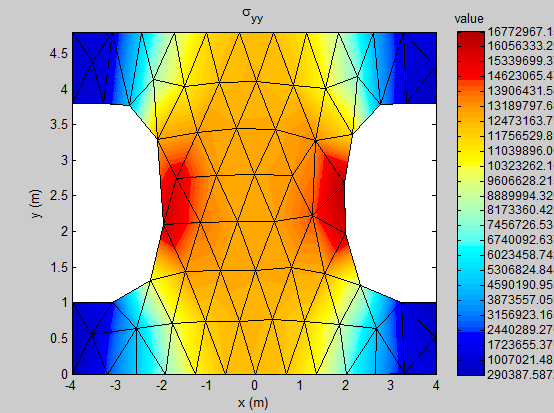
\includegraphics[width=\textwidth]{stress02.png}
		\caption{$L = 0.2 A$}
	\end{subfigure}
	\hfill
	\begin{subfigure}[b]{0.45\textwidth}
		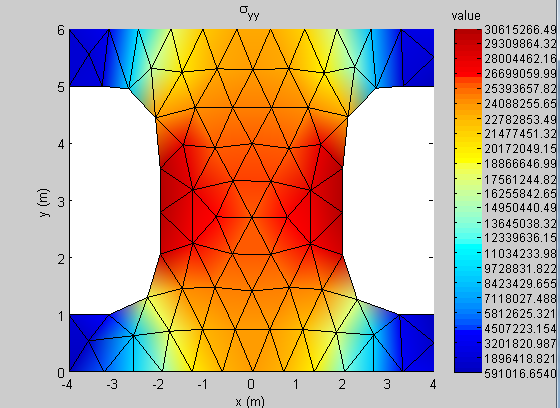
\includegraphics[width=\textwidth]{stress05.png}
		\caption{$L = 0.5 A$}
	\end{subfigure}
	\\
	\begin{subfigure}[b]{0.45\textwidth}
		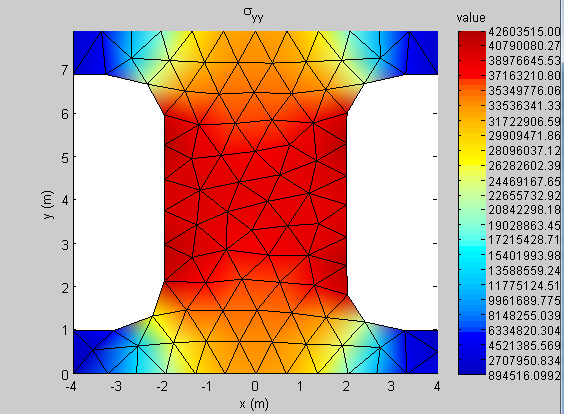
\includegraphics[width=\textwidth]{stress1.png}
		\caption{$L = 1 A$}
	\end{subfigure}
	\hfill
	\begin{subfigure}[b]{0.45\textwidth}
		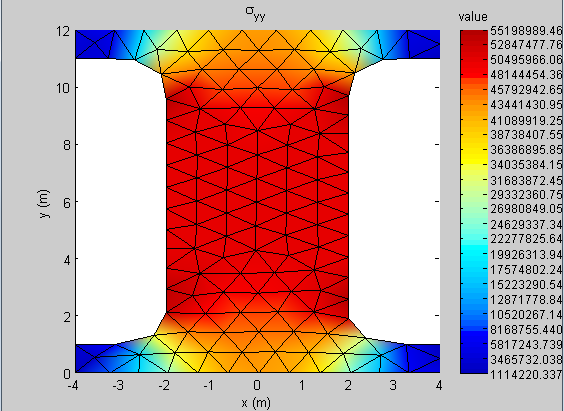
\includegraphics[width=\textwidth]{stress2.png}
		\caption{$L = 2 A$}
	\end{subfigure}
	\\
	\begin{subfigure}[b]{0.45\textwidth}
		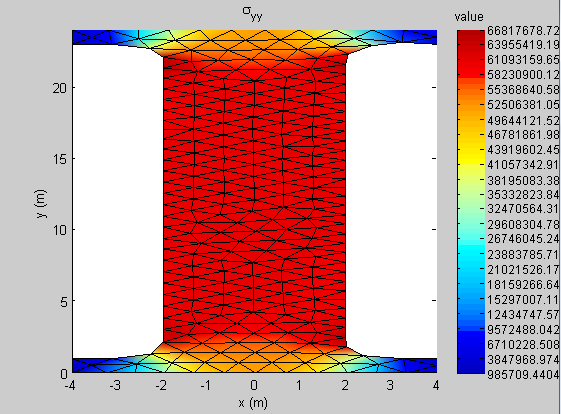
\includegraphics[width=\textwidth]{stress5.png}
		\caption{$L = 5 A$}
	\end{subfigure}
	\hfill
	\begin{subfigure}[b]{0.45\textwidth}
		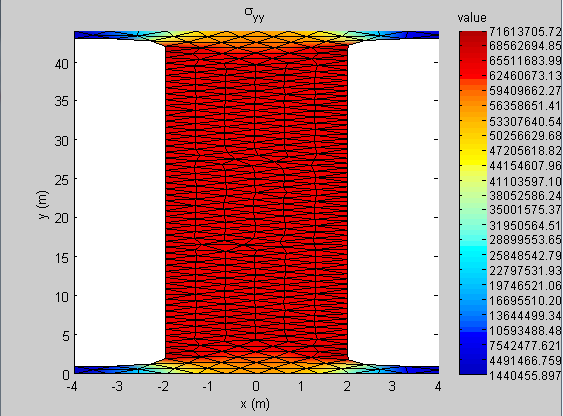
\includegraphics[width=\textwidth]{stress10.png}
		\caption{$L = 10 A$}
	\end{subfigure}
	\caption{$\sigma_{yy}$ distributions}
	\label{fig:stressdistp2}
\end{figure}



%----------------------------------------------------------------------------------------
%	PROBLEM 3
%----------------------------------------------------------------------------------------
\pagebreak
\section{Flat Plate with a Hole}

The results from the flat plate with a hole are as follows. Due to the fine sensitivity of the error to the mesh size, the median error for ten runs of each mesh size (0.03, 0.06, 0.2, 0.6, and 1). The results are in table \ref{tab:errortabp3}. 
The log-log plot of the error is seen in fig. \ref{fig:q3_errloglog}.\\\\
Notice that the error is not a straight line but rather jagged. It trends some what linear, and that is what was expected, and has a average slope around 0.5 and a curve fit slope closer to 1.0. Using linear interpolation the convergence rate 'p' can be found similarly to the discussion in class where $p = k + 1 -q$, where $k=1$ for linear interpolation and $q=1$ for the stress as it is a first derivative term from displacement. The resulting p is 1.0 which matches closely to the calculated slope of the error. 

\begin{table}[h]
\centering
	\begin{tabular}{c c c}
		Grid definition & Averaged Error [\%] \\
		\hline 
		0.03 & 4.971 \\
		0.06 & 11.289 \\
		0.2 & 11.992 \\
		0.6 & 36.370 \\
		1.0 & 46.276 \\
		\hline
	\end{tabular}
	\caption{Error at each grid definition}
	\label{tab:errortabp3}
\end{table}

\begin{figure}[h]
\centering
	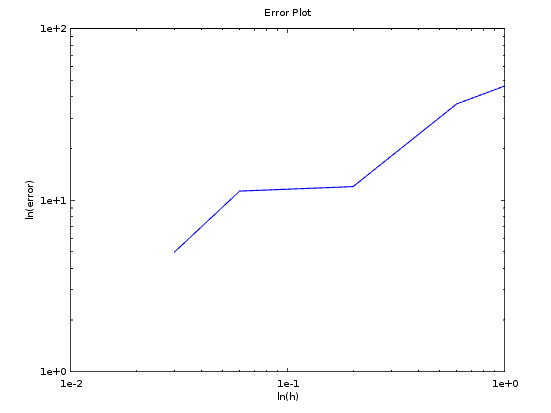
\includegraphics[scale=0.45]{q3_errloglog.png}
	\caption{Log-Log plot of error}
	\label{fig:q3_errloglog}
\end{figure}
%----------------------------------------------------------------------------------------

\end{document}
